\documentclass{article}

\usepackage{geometry}
% \geometry{left=3cm,right=3cm,top=3cm,bottom=3cm}

\usepackage{graphicx}
\usepackage{subcaption}

\usepackage{mathtools}
\usepackage{amssymb}

\usepackage{minted}
\setminted[haskell]{escapeinside=@@}
\newcommand{\hs}{\mintinline{haskell}}

\usepackage[hidelinks]{hyperref}
\usepackage[utf8]{inputenc}
\usepackage{enumitem}

\usepackage[
backend=biber
]{biblatex}
\addbibresource{bibliography.bib}

\renewcommand{\epsilon}{\varepsilon}
\newcommand{\eps}{\epsilon}
\newcommand{\overlay}{\oplus}
\newcommand{\connect}{\rightarrow}

\DeclarePairedDelimiter\abs{\lvert}{\rvert}%
\DeclarePairedDelimiter\norm{\lVert}{\rVert}%

% Swap the definition of \abs* and \norm*, so that \abs
% and \norm resizes the size of the brackets, and the 
% starred version does not.
\makeatletter
\let\oldabs\abs
\def\abs{\@ifstar{\oldabs}{\oldabs*}}
% 
\let\oldnorm\norm
\def\norm{\@ifstar{\oldnorm}{\oldnorm*}}
\makeatother

\title{Algebraic Graphs with Class}
\author{
  Christoph Madlener\\
  \texttt{\href{mailto:madlener@in.tum.de}{madlener@in.tum.de}}
}

\begin{document}

\maketitle
\begin{abstract}
  We give an overview of algebraic graphs as introduced by
  Mokhov~\cite{mokhov2017algebraic}. Algebraic graphs have a small and safe core
  of construction primitives, alongside a set of axioms, characterizing an
  algebra of graphs. They can be used to elegantly implement a graph
  transformation library employing functional programming. We also review the
  suitability of algebraic graphs for formal verification using Isabelle/HOL.
\end{abstract}

\section{Introduction}\label{sec:intro}
Graphs are a fundamental structure studied in depth by both mathematicians and
computer scientists alike. One very common definition states that a (directed)
graph is a tuple $G = (V,E)$, where $V$ is a set of vertices and $E \subseteq V
\times V$ is the set of edges. While this is a perfectly valid and natural
mathematical definition it is not necessarily suitable for implementation. This
can be illustrated by trying to directly translate this to Haskell:
\begin{minted}{haskell}
  data G a = G { vertices :: Set a, edges :: Set (a,a)}
\end{minted}
The value \hs{G {[1,2,3], [(1,2),(2,3)]}} then represents the graph $G =
(\{1,2,3\}, \{(1,2),(2,3)\})$, however \hs{G {[1,2], [(2,3)]}} does not
represent a consistent graph, as the edge refers to a non-existent node.
The state-of-the-art \texttt{containers} library implements graphs with
adjacency lists employing immutable arrays~\cite{king1995dfs}. The
consistency condition $E \subseteq V \times V$ is not checked statically though,
which can lead to runtime errors. \texttt{fgl}, another popular Haskell graph
library uses inductive graphs~\cite{erwig2001inductive}, also exhibiting partial
functions and potential for runtime errors due to the violation of consistency.

This lead Mokhov to conceive \textit{algebraic
  graphs}~\cite{mokhov2017algebraic}, a sound and complete representation for
graphs. They abstract away from graph representation details and characterize
graphs by a set of axioms. Algebraic graphs have a small safe core of graph
construction primitives and are suitable for implementing graph transformations.
These primitives are represented in the following datatype:
\begin{minted}{haskell}
  data Graph a = Empty
               | Vertex a
               | Overlay (Graph a) (Graph a)
               | Connect (Graph a) (Graph a)
\end{minted}
\hs{Empty} constructs the empty graph, \hs{Vertex} a graph with a single vertex
and no edges. \hs{Overlay} essentially is the union of two graphs and
\hs{Connect} additionally adds edges from all vertices from one graph to all
vertices of the other.

Alongside proper definitions for these primitives we will see
in~\autoref{sec:locale} that this is indeed a sound and complete graph
representation. We will also cover the algebraic structure (\ref{sec:algebra})
exhibited by these graphs and elegant graph transformations (\ref{sec:trafo})
based on a type class for the core. In~\autoref{sec:verification} we explore how
we can exploit the algebraic structure in verification using Isabelle/HOL.

In~\autoref{sec:deep} we will examine the deep embedding (i.e.\
the datatype as opposed to the type class of the preceding sections) regarding
applicability in practice and in verification. In~\autoref{sec:quotient} we
define a quotient type in Isabelle/HOL which in essence is a deep embedding
which satisfies the axioms.

In~\autoref{sec:conclusion} we conclude and give an outlook on possible future
work and open questions connected to algebraic graphs as presented.

\section{A type class for algebraic graphs}\label{sec:locale}
This section will cover most parts of the original paper by
Mokhov~\cite{mokhov2017algebraic}. The graph construction primitives of
algebraic graphs will be formally defined and their soundness and completeness
proven. Afterwards we will cover the algebraic structure inherent to these
primitives. As part of this we will introduce a type class in Haskell which
further abstracts from implementation details. We will also see that different
classes of graphs can be obtained by extending the set of axioms. Instances of
these different classes and a graph transformation library in Haskell are
provided. To conclude this section we will explore the suitability of this type
class for formal verification in Isabelle/HOL.

\subsection{The Core}\label{sec:core}
In the introduction we already briefly saw the four graph construction
primitives. Let us first define the set of (consistent) graphs $\mathcal{G}$
over a fixed universe of vertices $\mathbb{V}$. A graph $G \in \mathcal{G}$ can
then be represented as a tuple $G=(V,E)$ where $V \subseteq \mathbb{V}$ and $E
\subseteq V \times V$.
The four graph construction primitives
then are defined as follows. The \textit{empty} graph, denoted $\eps$ is
simply the tuple $(\emptyset, \emptyset)$ which is clearly consistent, hence
$\eps \in \mathcal{G}$. Graphs with a single \textit{vertex} $v \in
\mathbb{V}$ and no edges, i.e.\ $(\{v\}, \emptyset)$  denoted by just $v$, are also
clearly consistent, hence $v \in \mathcal{G}$. The binary operations
\textit{overlay} and \textit{connect}, denoted by $\overlay$ and $\connect$
respectively, allow constructing larger graphs. Their definitions are
\begin{align*}
  (V_1, E_1) \overlay (V_2, E_2) &\coloneqq (V_1 \cup V_2, E_1 \cup E_2)\\
  (V_1, E_1) \connect (V_2, E_2) &\coloneqq (V_1 \cup V_2, E_1 \cup E_2 \cup V_1 \times V_2)
\end{align*}
So overlay is just the union of two graphs, while connect also adds an edge from
each vertex of the ``left'' graph to each vertex of the ``right'' graph. It is
straightforward to see that if $G_1 \in \mathcal{G}$ and $G_2 \in \mathcal{G}$
then also $G_1 \overlay G_2 \in \mathcal{G}$ and $G_1 \connect G_2 \in
\mathcal{G}$. In combination with the consistency of $\eps$ and of single vertex
graphs this already proves that algebraic graphs are a consistent
representation for graphs. The completeness of this representation, i.e.\ for
each $G \in \mathcal{G}$ there is an algebraic graph expression representing it,
is shown in the next subsection. Both of these facts were also formally proven in
Isabelle/HOL as part of~\autoref{sec:verification}.

As we will shortly see in~\autoref{sec:algebra} overlay and connect are somewhat
related to addition and multiplication, hence, we give connect a higher precedence
than overlay. Let us consider some examples to develop some intuition for the
primitives. They are illustrated in~\autoref{fig:construction}.
\begin{enumerate}[label=(\alph*)]
\item $1 \overlay 2 = (\{1,2\}, \emptyset)$
\item $1 \connect 2 = (\{1,2\}, \{(1,2)\})$
\item $1 \connect 2 \overlay 3 = (\{1,2,3\}, \{(1,2), (1,3)\})$
\item $1 \connect 2 \overlay 2 \connect 3 = (\{1,2,3\}, \{(1,2), (2,3)\})$
\end{enumerate}
\begin{figure*}
  \centering
  \begin{subfigure}[b]{0.3\linewidth}
    \centerline{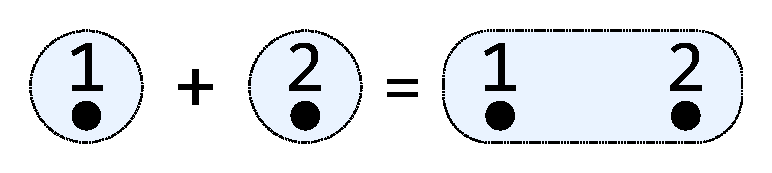
\includegraphics[scale=0.27]{fig/ex-a.pdf}}
    \vspace{-2.4mm}
    \caption{$1 \overlay 2$}
    \centerline{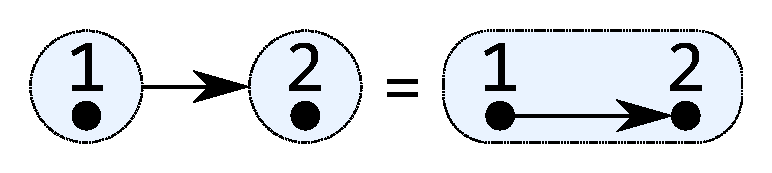
\includegraphics[scale=0.27]{fig/ex-b.pdf}}
    \vspace{-2.4mm}
    \caption{$1 \connect 2$}
  \end{subfigure}
  \begin{subfigure}[b]{0.3\linewidth}
    \centerline{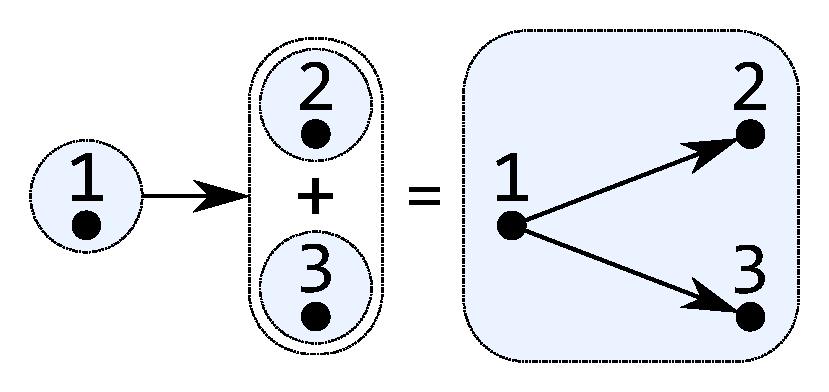
\includegraphics[scale=0.27]{fig/ex-c.pdf}}
    \vspace{-1mm}
    \caption{$1 \connect (2 \overlay 3)$}
  \end{subfigure}
  \hspace{3mm}
  \begin{subfigure}[b]{0.3\linewidth}
    \centerline{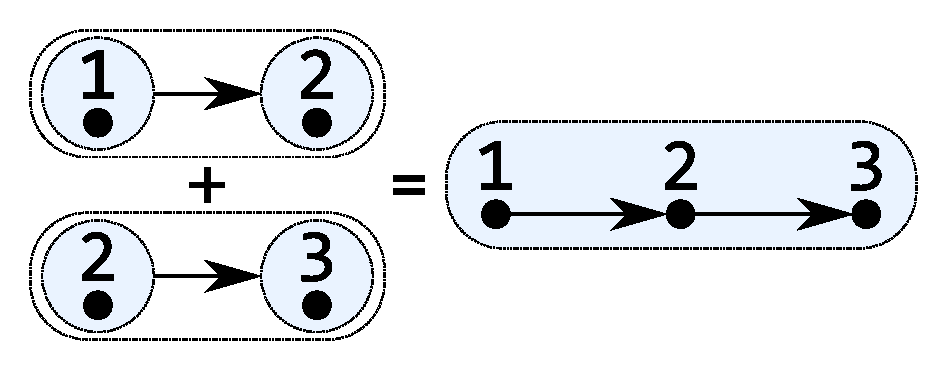
\includegraphics[scale=0.27]{fig/ex-e-new.pdf}}
    \vspace{-1mm}
    \caption{$1 \connect 2 \overlay 2 \connect 3$}
  \end{subfigure}
  \caption{Examples of graph construction. The overlay and connect operations
    are denoted by $\overlay$ and $\connect$, respectively. Illustrations
    from~\cite{mokhov2017algebraic}.\label{fig:construction}} 
\end{figure*}

We already saw how to deeply embed these graph construction primitives in a
datatype. For greater reusability the following type class can be defined.
\begin{minted}{haskell}
  class Graph g where
      type Vertex g
      empty :: g
      vertex :: Vertex g -> g
      overlay :: g -> g -> g
      connect :: g -> g -> g
\end{minted}
The associated type \hs{Vertex g} represents the universe of vertices
$\mathbb{V}$, the remainder of the type class corresponds to $\eps$, single
vertex graphs, $\overlay$ resp.\ $\connect$.

At this point we will only introduce some very basic functions for constructing
graphs. More advanced constructions and transformations will be given
in~\autoref{sec:trafo}. A graph with a single edge is obtained by simply
connecting two vertices:
\begin{minted}{haskell}
  edge :: Graph g => Vertex g -> Vertex g -> g
  edge u v = (vertex u) `connect` (vertex v)
\end{minted}
A graph with only isolated vertices can be constructed from a list of vertices
as follows:
\begin{minted}{haskell}
  vertices :: Graph g => [Vertex g] -> g
  vertices vs = foldr overlay empty . map vertex
\end{minted}
Replacing \hs{overlay} with \hs{connect} in \hs{vertices} leads to a (directed)
clique. Later we will also consider undirected graphs. In that context this
function actually builds a fully connected graph on the given list of vertices.
\begin{minted}{haskell}
  clique :: Graph g => [Vertex g] -> g
  clique vs = foldr connect empty . map vertex
\end{minted}
Following and extending this approach leads to a safe and fully polymorphic
graph transformation library for any concrete graph representation (e.g.\ graphs
in \texttt{containers} or \texttt{fgl}) instantiating this class.

\subsection{Algebraic Structure}\label{sec:algebra}
Before turning to more advanced graph constructions we will observe the
algebraic structure of the primitives. It turns out that overlay and connect
almost form a semiring over graphs:
\begin{itemize}
\item $(\mathcal{G}, \overlay, \eps)$ is an idempotent commutative monoid
\item $(\mathcal{G}, \connect, \eps)$ is a monoid
\item $\connect$ distributes over $\overlay$
\end{itemize}
The shared identity and the missing annihilating zero for $\connect$
(i.e.\ $x \connect 0 = 0$) are the only difference. There is also the following
\textit{decomposition law}, as illustrated in~\autoref{fig:axioms}(b).
\[
  x \connect y \connect z = x \connect y \overlay x \connect z \overlay y \connect z
\]
Using decomposition we can actually prove some of the above properties, leading
to the following minimal set of axioms characterizing directed graphs:
\begin{itemize}
\item $(G, \overlay)$ is a commutative semigroup
\item $(G, \connect, \eps)$ is a monoid
\item $\connect$ distributes over $\overlay$, i.e.\ $x \connect (y \overlay z)
  = x \connect y \overlay x \connect z$ and $(x \overlay y) \connect z = x
  \connect z \overlay y \connect z$
\item decomposition: $x \connect y \connect z = x \connect y \overlay x
  \connect z \overlay y \connect z$ 
\end{itemize}
\begin{figure*}
  \begin{subfigure}[b]{0.4\linewidth}
    \centerline{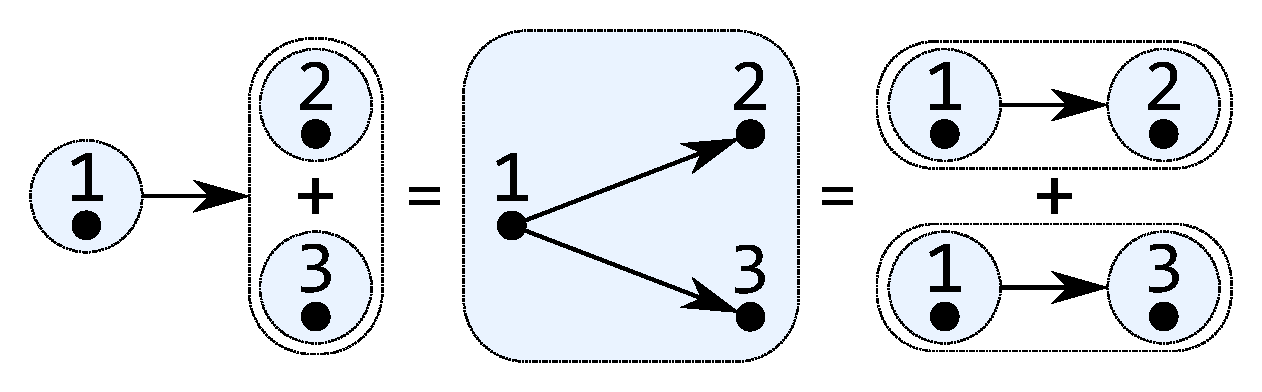
\includegraphics[scale=0.24]{fig/ax-distributivity.pdf}}
    \caption{Distributivity: $1 \connect (2 \overlay 3) = 1 \connect 2 \overlay
      1 \connect 3$ }
  \end{subfigure}
  \hspace{12mm}
  \begin{subfigure}[b]{0.5\linewidth}
    \centerline{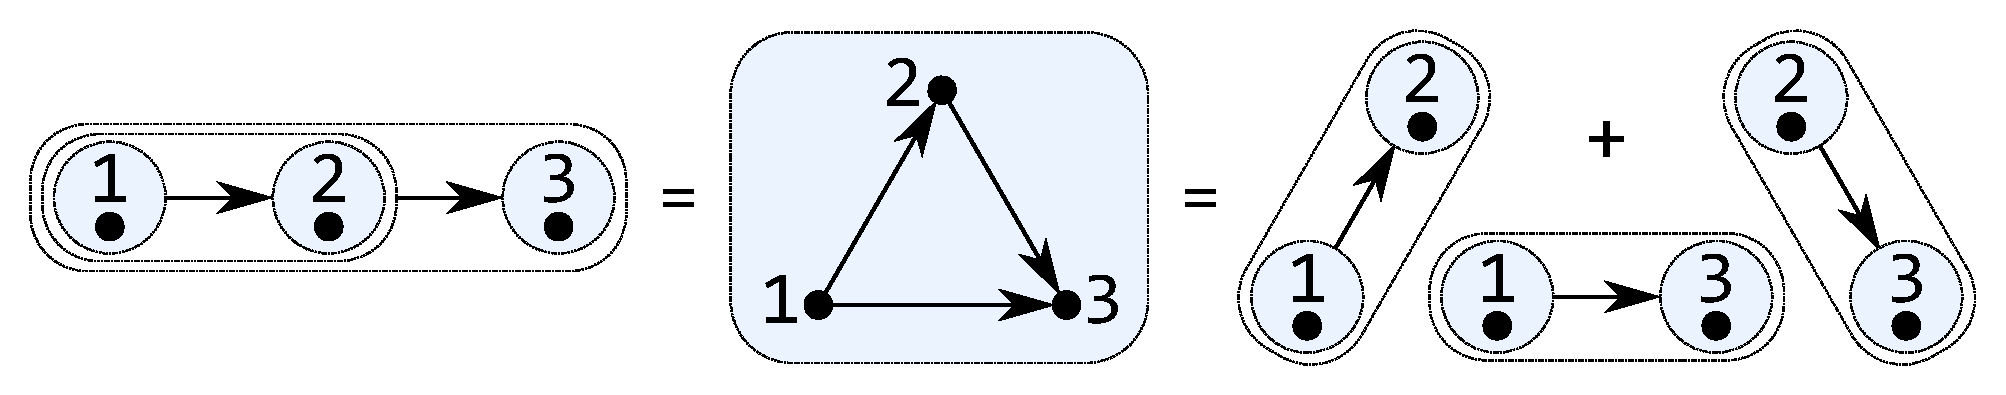
\includegraphics[scale=0.24]{fig/ax-decomposition.pdf}}
    \caption{Decomposition: $1 \connect 2 \connect 3 = {1 \connect 2} \overlay
      1 \connect 3 \overlay 2 \connect 3$}
  \end{subfigure}
  \vspace{-1mm}
  \caption{Two axioms of the algebra of graphs. Illustrations from~\cite{mokhov2017algebraic}.\label{fig:axioms}}
\end{figure*}
One can easily check that the definitions of the primitives given
in~\autoref{sec:core} satisfy these axioms. At this point let us consider the
completeness of algebraic graphs. For any graph $G=(V,E)$ the following function
builds it using the four construction primitives:
\begin{minted}{haskell}
  graph :: Graph g => [Vertex g] -> [(Vertex g, Vertex g)] -> g
  graph vs es = overlay (vertices vs) (edges es)
\end{minted}
The \hs{edges} function generalizes \hs{edge} to a list of edges:
\begin{minted}{haskell}
  edges :: Graph g => [(Vertex g, Vertex g)] -> g
  edges = foldr overlay empty . map (uncurry edge)
\end{minted}
This was also formally proven in Isabelle/HOL (see~\autoref{sec:verification}).

Mokhov also follows a standard approach of defining a partial order $(\preceq)$ for the
idempotent overlay operation as $x \preceq y \iff x \overlay y = y$. This is indeed
a partial order under the graph axioms (i.e.\ it is reflexive, antisymmetric and
transitive). In fact this partial order can actually be used as a definition for
the subgraph relation, denoted by $\subseteq$:
\[
  x \subseteq y \coloneqq x \preceq y \iff x \overlay y = y
\]

So far we only considered directed graphs. Undirected graphs can be
obtained from the same construction primitives as directed graphs. It suffices
to modify the underlying axioms. In the case of undirected graphs this can be
achieved by making connect commutative (then denoted by $\leftrightarrow$),
i.e.\ $x \leftrightarrow y = y \leftrightarrow x$. By introducing this axiom we
can prove some of the axioms of directed graphs. Hence, undirected graphs are
characterized by the following minimal set of axioms:
\begin{itemize}
\item $(\mathcal{G}, \oplus)$ is a commutative semigroup
\item $\leftrightarrow$ is commutative and has $\eps$ as the identity
\item left distributivity: $x \leftrightarrow (y \oplus z) = x \leftrightarrow
  y \oplus x \leftrightarrow z$
\item left decomposition: $(x \leftrightarrow y) \leftrightarrow z = x
  \leftrightarrow y \oplus x \leftrightarrow z \oplus y \leftrightarrow z$
\end{itemize}
By choosing different additional axioms, other classes of graphs can be
characterized. Some examples are reflexive graphs (i.e.\ each vertex has a
self-loop), transitive graphs (as in dependency graphs), and the combination
thereof; preorders. Combining undirected graphs and reflexive graphs yields
equivalence relations. It is even possible to define hypergraphs of arbitrary
(but fixed) order by replacing the decomposition law with another suitable
axiom~\cite{mokhov2017algebraic}.

In summary the algebraic approach to graph representation has a small and safe
core of construction primitives. Pairing these primitives with suitable sets of
axioms leads to a highly flexible representation for graphs.

\subsection{Graph Transformation Library}\label{sec:trafo}
Based on this core type class, Mokhov implements what he refers to as a graph
transformation library\footnote{Algebraic graphs on hackage:
  \texttt{\href{http://hackage.haskell.org/package/algebraic-graphs}{http://hackage.haskell.org/package/algebraic-graphs}}}.
In order to understand the following constructions and transformations better,
we follow the approach of Mokhov and first define instances for the type class
\hs{Graph}. Recall the attempt from the introduction to directly translate the
graph representation $G=(V,E)$ into the Haskell datatype \hs{G}. We will now
define a \hs{Graph} instance for that datatype, while realizing that more
generally it can be used to represent relations on some domain (hence the renaming
to \hs{Relation}).
\begin{minted}{haskell}
  data Relation a = R { domain :: Set a, relation :: Set (a, a)} deriving Eq

  instance Ord a => Graph (Relation a) where
    type Vertex (Relation a) = a
    empty       = R Set.empty Set.empty
    vertex  x   = R (singleton x) Set.empty
    overlay x y = R (domain x `union` domain y) (relation x `union` relation y)
    connect x y = R (domain x `union` domain y) (relation x `union` relation y `union'
      fromAscList [ (a, b) | a <- elems (domain x), b <- elems (domain y) ])
\end{minted}
Mokhov also defines a \hs{Num} instance for \hs{Relation} which enables the use
of \hs{+} and \hs{*} as shortcuts for \hs{overlay} resp.\ \hs{connect}.

The given \hs{Graph} instance for \hs{Relation} satisfies the axioms of directed
graphs, as was argued in~\autoref{sec:core}. Obtaining \hs{Graph} instances
which satisfy the axioms for undirected graphs (or other classes of graphs) is
also straightforward: One can simply wrap \hs{Relation} in a \hs{newtype} and
define a custom \hs{Eq} instance. An example for undirected graphs (in this case
think of symmetric directed graphs) is given.
\begin{minted}{haskell}
  newtype Symmetric a = S (Relation a) deriving (Graph, Num)

  instance Ord a => Eq (Symmetric a) where
    S x == S y = symmetricClosure x == symmetricClosure y
\end{minted}
It is also sensible to introduce subclasses like \hs{class Graph g => UndirectedGraph g}
to reflect the class of graph we are working with in the type system, and thus,
increase type safety.

Equipped with these two instances let us now actually consider graph
constructions and transformations made possible with the core type class. Simple
examples include constructing a \textit{path} from a list of vertices, which
then can be easily extended to a \textit{circuit}:
\begin{minted}{haskell}
  path :: Graph g => [Vertex g] -> g
  path []  = empty
  path [x] = vertex x
  path xs = edges $ zip xs (tail xs)

  circuit :: Graph g => [Vertex g] -> g
  circuit [] = empty
  circuit xs = path (xs ++ [head xs])
\end{minted}
Mokhov also gives functions for constructing \textit{star} graphs (i.e.\ a
center vertex connected to a set of leaves) and for building graphs from
\hs{Tree}s and \hs{Forest}s from the \texttt{containers} library.

More interesting applications include the implementation of a zero time
graph transposition using a \hs{newtype} wrapper~\cite{mokhov2017algebraic}:
\begin{minted}{haskell}
  newtype Transpose g = T { transpose :: g } deriving Eq

  instance Graph g => Graph (Transpose g) where
    type Vertex (Transpose g) = Vertex g
    empty       = T empty
    vertex      = T . vertex
    overlay x y = T $ overlay (transpose x) (transpose y)
    connect x y = T $ connect (transpose y) (transpose x)
\end{minted}
Although for certain representations it is possible to get an $\mathcal{O}(1)$
transpose operation (e.g.\ by setting a transposed flag), for many typical
representations the whole graph has to be traversed, resulting in
$\mathcal{O}(\abs{V} + \abs{E})$ time.

More sophisticated transformations can be implemented using the following
\hs{Functor}-like \hs{newtype} wrapper. The function \hs{gmap} takes a function
\hs{a -> b} and a graph with vertices of type \hs{a} and produces a graph with
vertices of type \hs{b} polymorphically.
\begin{minted}{haskell}
  newtype GraphFunctor a = F { gfor :: forall g. Graph g => (a -> Vertex g) -> g }

  instance Graph (GraphFunctor a) where
    type Vertex (GraphFunctor a) = a
    empty       = F $ \_ -> empty
    vertex  x   = F $ \f -> vertex (f x)
    overlay x y = F $ \f -> overlay (gmap f x) (gmap f y)
    connect x y = F $ \f -> connect (gmap f x) (gmap f y)

  gmap :: Graph g => (a -> Vertex g) -> GraphFunctor a -> g
  gmap = flip gfor  
\end{minted}
Interestingly this can be used to merge vertices fulfilling some predicate
\hs{p} by mapping them to a single vertex:
\begin{minted}{haskell}
  mergeVertices :: Graph g => (Vertex g -> Bool)
    -> Vertex g -> GraphFunctor (Vertex g) -> g
  mergeVertices p v = gmap $ \u -> if p u then v else u
\end{minted}
In the original paper \hs{gmap} is then used further to construct rather
sophisticated graphs fully polymorphically~\cite{mokhov2017algebraic}.

Mokhov also goes on to introduce a \hs{Monad}-like \hs{newtype} wrapper. The
\hs{bind} in the context of graphs allows to replace each vertex with a
(possibly empty) subgraph. This can be used to both remove and split vertices.
\begin{minted}{haskell}
  newtype GraphMonad a = M { bind :: forall g. Graph g => (a -> g) -> g }

  instance Graph (GraphMonad a) where
    type Vertex (GraphMonad a) = a
    empty       = M $ \_ -> empty
    vertex x    = M $ \f -> f x
    overlay x y = M $ \f -> overlay (bind x f) (bind y f)
    connect x y = M $ \f -> connect (bind x f) (bind y f)
\end{minted}
Removing a vertex with \hs{bind} can be generalized to a function \hs{induce},
which only keeps vertices satisfying some predicate \hs{p}.
\begin{minted}{haskell}
  induce :: Graph g => (Vertex g -> Bool) -> GraphMonad (Vertex g) -> g
  induce p g = bind g $ \v -> if p v then vertex v else empty
\end{minted}
Splitting a vertex works by replacing that vertex with a graph containing the
desired vertices.
\begin{minted}{haskell}
  splitVertex :: (Graph g, Eq (Vertex g)) => Vertex g -> [Vertex g] 
    -> GraphMonad (Vertex g) -> g
  splitVertex v vs g = bind g $ \u -> if u == v then vertices vs else vertex u
\end{minted}
Mokhov then defines yet another \hs{newtype} wrapper utilizing \hs{bind} to
remove edges. He also showcases the construction capabilities of the presented
library by constructing de Bruijn graphs (a rather sophisticated type of graph
occurring frequently occurring in computer engineering and bioinformatics)
completely polymorphically. These definitions are omitted here for brevity.

The presented material on the given type class gives an overview of an elegant,
reusable and polymorphic graph construction and transformation library. Note
that in the available \texttt{hackage} library for algebraic graphs the
\hs{newtype} wrappers for graph transformation are not implemented in the
presented type class. Instead there is a higher-kinded type class which is based
on \hs{MonadPlus}, but has fewer instances~\cite{mokhov2017algebraic}.

\subsection{Verification}\label{sec:verification}
We have now seen how to implement a polymorphic graph transformation library in
Haskell using the core type class. Mokhov proposes that algebraic graphs and
their axiomatic characterization are suitable for formal verification as they
enable equational reasoning. Some
simple statements (like $\hs{vertices xs} \subseteq \hs{clique xs}$) are given
accompanied by an Agda formalization\footnote{available at
  \texttt{\href{https://github.com/snowleopard/alga-theory}{https://github.com/snowleopard/alga-theory}}}.
For the examples in that formalization the claim obviously holds.

To experiment further we first formalized the available material in
Isabelle/HOL~\cite{isabelle}.
This formalization\footnote{available at
  \texttt{\href{https://github.com/cmadlener/algebraic_graphs}{https://github.com/cmadlener/algebraic\_graphs}}}
involves the definition of a \textit{locale}, which for the
purposes of this paper can be thought of as a type class which can be equipped
with axioms. Proving the statements from the paper in Isabelle/HOL works
conveniently.

Noschinski formalized graph theory in
Isabelle/HOL~\cite{GraphTheory-AFP}. A part of that is essentially the standard
representation of a graph as a tuple $G=(V,E)$ (i.e.\ a locale with a
consistency axiom). Instantiating a locale (which can be likened to
instantiating a type class in Haskell) requires to prove the axioms attached to
it. Using the definitions from~\autoref{sec:core} for the primitives it is
straightforward to instantiate the algebraic graph locale for the tuple
representation. We also formally prove that the graph construction primitives only
produce consistent graphs. A proof for the completeness of the primitives is
given as well (as long as we accept that the tuple representation is a
\textit{complete} graph representation).

As the statements in the original paper were of very limited scope, we 
define and reason about more \textit{advanced} graph theoretic concepts: We
introduce (vertex) walks and the notion of reachability on algebraic graphs.
First impressions suggest that it is feasible to base more sophisticated
formalizations of graph theory on algebraic graphs. Although we suspect that
some additional axiom(s) may be required to make for \textit{interesting} graph
theory; as it stands the statement $\eps \neq \hs{vertex u}$ for a $u \in
\mathbb{V}$ is unprovable. This is further illustrated by the fact that we can
instantiate the algebraic graph locale with the unit type.

This is an interesting direction for future work for a related reason that the
type class is interesting in Haskell: The type class forms the basis for 
a polymorphic graph transformation library, whereas the locale can be
seen as a \textit{polymorphic} graph formalization library. Any lemma we can prove
using the locale axioms becomes available to any graph representation
instantiating it. This obviously becomes more interesting the more material is
available in the locale. Haslbeck et al.\ chose a similar approach to implement
and verify Kruskal's algorithm independent of the concrete graph
representation~\cite{Kruskal-AFP}.

\section{Deep Embedding}\label{sec:deep}
Up until this point we were mainly concerned with exploiting the algebraic
structure of graphs for polymorphic graph constructions and transformations, and
for formal verification. However, that the deep embedding of the
construction primitives in a datatype is interesting in itself. Recall the
definition from the introduction:
\begin{minted}{haskell}
  data Graph a = Empty
               | Vertex a
               | Overlay (Graph a) (Graph a)
               | Connect (Graph a) (Graph a)
\end{minted}
An instance for the type class can be defined easily, however, we cannot use the
derived \hs{Eq} instance for the datatype, as it would violate the graph axioms.
One solution is to fold the deep embedding into a concrete graph representation to
obtain a law-abiding \hs{Eq} instance:
\begin{minted}{haskell}
  fold :: Graph g => Graph (Vertex g) -> g
  fold Empty         = empty
  fold (Vertex  x  ) = vertex x
  fold (Overlay x y) = overlay (fold x) (fold y)
  fold (Connect x y) = connect (fold x) (fold y)

  instance Ord a => Eq (Graph a) where
    x == y = fold x == (fold y :: Relation a)
\end{minted}
This approach is also currently implemented in the library available on
\texttt{hackage}. However, this is not ideal for multiple reasons. Coupling the
datatype to some other graph representation merely for equality checks is
inconvenient at best. More interestingly algebraic graphs can compactly
represent dense graphs. Consider the graph \hs{clique [1..n]}, which is linear
in size in the deep embedding, while it is quadratic when stored as a
\hs{Relation}. Requiring to fully expand graphs to check equality voids this
advantage. A promising approach to alleviate this issue is the \textit{modular
  graph decomposition}~\cite{mcconnell2005linear}, as it allows to minimize
algebraic graph expressions. It remains an open question if this decomposition
can be computed efficiently directly on the deep embedding.

More interesting questions for future work come up in connection with the deep
embedding. Currently only the transformations presented with the type class, i.e.\
transpose, as well as anything that can be done using the corresponding versions
of \hs{gmap} and \hs{bind}, are implemented directly on the deep embedding. No
known efficient implementations of fundamental graph algorithms, like
depth-first-search, that work directly on the deep embedding are
known~\cite{mokhov2017algebraic}. The library therefore resorts to converting
algebraic graph expressions to an adjacency map and uses algorithms
for those.

An immediate application which can be more efficient in space using
algebraic graphs that comes to mind is search, however, only in best case
examples, i.e.\ where only a small part of the graph has to be expanded. This is
due to the fact that the neighborhood of a vertex in an algebraic graph
expression can be computed in linear (in the size of the graph expression) time
and space. We already saw that the algebraic graph representation can be
significantly smaller than conventional representations.

Some benchmarks were performed (on an earlier version of the library) to compare
its performance to \texttt{containers} and \texttt{fgl} (and one other
representation). The results are mixed; depending on the area of application,
algebraic graphs may be competitive in performance, or in some cases, orders of
magnitudes slower. For the full results refer to the benchmark suite
repository\footnote{available at
  \texttt{\href{https://github.com/haskell-perf/graphs}{https://github.com/haskell-perf/graphs}}}.
\subsection{Verification}\label{sec:quotient}
We were also interested in using the deep embedding in formal verification using
Isabelle/HOL. Hence, we formalized most of the material from the library. This
feat turned out nicely, as the inductive datatype definition of the deep
embedding enables proofs by induction.

In the Haskell implementation of the deep embedding we already saw that
structural equality does not satisfy the axioms. There we can define a custom
\hs{Eq} instance to obtain a law-abiding datatype. In Isabelle/HOL we can follow
a similar approach, which results in a \texttt{quotient\_type}, which can be
thought of as an equivalence class construction on the raw datatype. For the
moment the equivalence is based on the tuple representation by Noschinski
mentioned in~\autoref{sec:verification}. Again, the minimization of algebraic
graph expressions for an equivalence relation on algebraic graphs, decoupled
from any other graph representation, is desirable.

The quotient type also allows us to formally prove that it satisfies the axioms,
by instantiating the locale. It also paves the way for further formalization
efforts on the deep embedding. However, this only becomes really interesting
with more future work, i.e.\ if algorithms that work directly on the deep
embedding or other advanced usages of it can be found (in other words, if there
is more material to formalize).

\section{Conclusion}\label{sec:conclusion}
We saw a novel approach to representing graphs, which is especially suitable for
functional programming. It allows for safe, polymorphic and elegant graph
constructions and transformations. Algebraic graphs also lend themselves nicely
to formal verification.

The alert reader might have noticed that the given primitives can only be used
to represent unlabeled graphs. Mokhov extended the algebraic graph library to
also represent edge-labeled graphs. There is no published material on this yet
(besides the source code), for more information refer to the talk by Mokhov
during Haskell eXchange 2018\footnote{available at
  \texttt{\href{https://skillsmatter.com/skillscasts/12361-labelled-algebraic-graphs}{https://skillsmatter.com/skillscasts/12361-labelled-algebraic-graphs}}}.

Algebraic graphs as presented have been successfully used in practice, e.g.\ for
asynchronous circuit design~\cite{beaumont2017high} and acceleration of graph
processing using FPGAs~\cite{mokhov2019language}. These are examples for which
the available transformations are sufficient. An important direction for future
research is going beyond those (relatively simple) transformations. That means
to find and formulate algorithms either inside the core type class or directly
on the deep embedding. Berghammer et. al~\cite{berghammer2020relational}
successfully employ algebraic approaches to formally verify graph algorithms.
However, they are using an algebra of relations as opposed to the one here
defined using graph construction primitives. Dolan~\cite{dolan2013fun} uses an
algebra on adjacency matrices to find paths in graphs.
Mokhov himself postulates that the algebraic approach allows to formulate graph
algorithms as systems of equations with unknowns. This approach may also be a
way to find novel graph algorithms.

\printbibliography

\end{document}